% Beamer Presentation and Lecture Note Template
% Version 0.1
% by Paul Vesey

\mode<presentation> {
\usetheme{Antibes}
\setbeamercovered{invisible}
\setbeamertemplate{footline}[frame number]
\setbeamertemplate{navigation symbols}{} 
}

\usepackage{eurosym}
\usepackage{graphicx}
\usepackage{wasysym}
\usepackage{hyperref}
\usepackage{amsmath}
\usepackage{amssymb}
\usepackage{mathtools}
\usepackage{tikz}
\usepackage{pgf}
\usepackage{pgfplots}
\usepackage{pxfonts}
\usepackage{textcomp}
\usepackage{verbatim}
\usepackage{color}
\usepackage{xcolor}
\usepackage{fix-cm}


\author{Paul Vesey}
\institute[TUS]
{
Technological University of the Shannon \\
\medskip
{\emph{paul.vesey@tus.ie}}
}
\date{Autumn 2022}



\title[Project Management]{Project Procurement Management}



\begin{document}
%
\usetikzlibrary{arrows}
\usepgflibrary{patterns}

\tableofcontents
\newpage



\begin{frame}
\titlepage
\end{frame}\begin{center}\line(1,0){250}\end{center}
%
%








\section{Project Procurement Management}

\subsection{Introduction}


\begin{frame}
\frametitle{Project Procurement Management}
\begin{itemize}
	\item Project Procurement Management includes the processes to purchase or acquire the products, services, or results needed from outside the project team to perform the work.
	\item Project Procurement Management includes the contract management and change control processes required to administer contracts or purchase orders.
\end{itemize}
\end{frame}\begin{center}\line(1,0){250}\end{center}



\begin{frame}
\frametitle{Project Procurement Management \hfill\hfill Proceses} 
\textbf{Plan Procurements}
		\begin{itemize}
			\item What, When and How - Documenting requirements and identifying potential sellers
		\end{itemize}
\textbf{Conduct Procurements}
		\begin{itemize}
			\item Request Seller Responses
		\end{itemize}
\textbf{Obtaining information, bids, quotations, proposals}
		\begin{itemize}
			\item Select Sellers
			\item Reviewing offers, choosing potential sellers, negotiating written contract with sellers
		\end{itemize}
\textbf{Administer Procurements}
		\begin{itemize}
			\item Managing Contract Relationships; reviewing and documenting seller performance; change management
		\end{itemize}
\textbf{Close Procurements}
		\begin{itemize}
			\item Completing and Settling each contract
		\end{itemize}
\end{frame}\begin{center}\line(1,0){250}\end{center}




\begin{frame}
\frametitle{Contractual Obligation}
\textbf{Contract}
\begin{itemize}
	\item Legally Binding
	\item Product, Service, Result, in exchange for Consideration
	\item Can be simple or complex
\end{itemize}
\begin{itemize}
	\item All contracts should be tailored to the specific needs of the project;\\
	\item Contracts require a more rigorous internal approval procedures\\
	\item Contracts present an opportunity for the performing organisation to avoid; mitigate; or transfer risk.\\
	\item When using standard forms of contract (MF1, FIDIC, etc.), any amendments need to be very carefully considered.
			\begin{itemize}
				\item Change may introduce unanticipated errors
			\end{itemize}
\end{itemize}
\end{frame}\begin{center}\line(1,0){250}\end{center}



\begin{frame}
\frametitle{Contracts}
\begin{itemize}
	\item Complex Projects typically include multiple contracts.
	\item These contracts can come into effect and be discharged at any time during the project
	\item The buyer-seller relationship can exist at many levels on any one project
	\item Sellers will typically manage their work as a project; unless their work is restricted to supply only
\end{itemize}
\end{frame}\begin{center}\line(1,0){250}\end{center}




\begin{frame}
\frametitle{Plan Procurements}
\textbf{Part of the Planning Process Group}
\begin{figure}
	\centering
		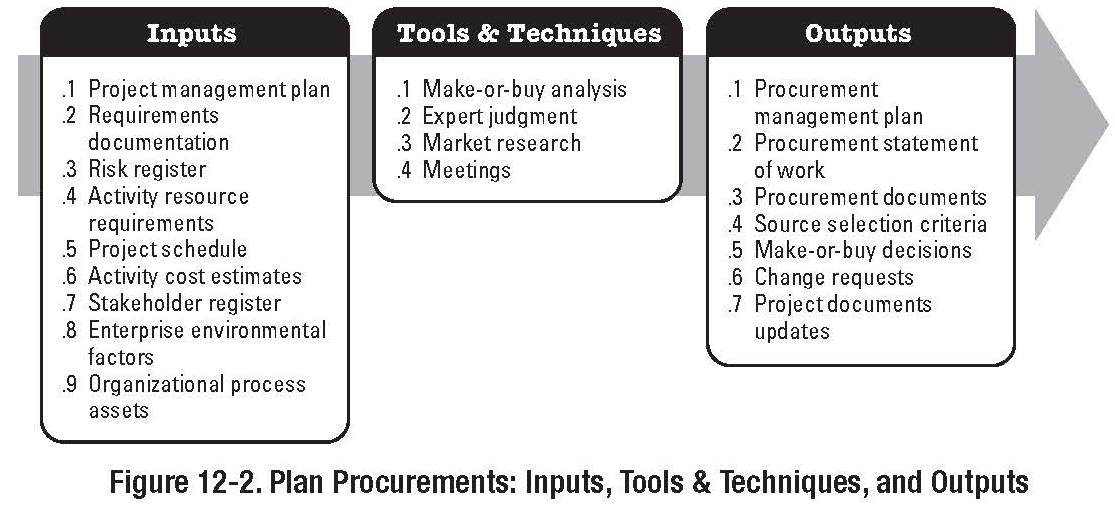
\includegraphics[width = 10cm]{images/Fig12-2.jpg}
	\label{fig:12-2}
\end{figure}
\end{frame}\begin{center}\line(1,0){250}\end{center}



\begin{frame}
\frametitle{Plan Procurements}
\begin{itemize}
	\item Identifies which project needs can best be met by purchasing or acquiring products, services or results from outside the project organisation, and which project needs can be accomplished by the project team
	\item Also includes detailing who is responsible for obtaining and holding permits, licences, etc. - i.e. main contractor or sub-contractor
	\item The process also includes reviewing the risks involved in each make-or-buy decision; reviewing the type (form) of contract that will be used for mitigating, avoiding or transferring risk
\end{itemize}
\end{frame}\begin{center}\line(1,0){250}\end{center}



\begin{frame}
\frametitle{Plan Purchases and Acquisitions \hfill\hfill Inputs (Incomplete list)}
\textbf{Enterprise Environmental Factors}
		\begin{itemize}
			\item Market Place Conditions
			\item Availability of products and services
		\end{itemize}
\textbf{Organisational Process Assets}
		\begin{itemize}
			\item Formal and Informal procurement policies
			\item Approval procedures; approved suppliers; contract terms
		\end{itemize}
\textbf{Project Scope Statement - information on:}
		\begin{itemize}
			\item How much money is available
			\item Required by dates
			\item Health \& Safety, Security, Performance, Insurances, etc.
			\item Deliverables and Acceptance Criteria
		\end{itemize}
\end{frame}\begin{center}\line(1,0){250}\end{center}


\begin{frame}
\frametitle{Plan Purchases and Acquisitions \hfill\hfill Inputs (Incomplete list)}
\begin{itemize}
 \item WBS \& Dictionary: Provides the relationship amongst components of the project and detailed description of the works within each WBS element.
 \item PM Plan: Provides guidance and direction for procurement planning
 \item Risk Register: Risk Related contractual Agreements
 \item Activity Resource Requirements
 \item Project Schedule
 \item Activity  Cost Estimates
 \item Cost Baseline
\end{itemize}
\end{frame}\begin{center}\line(1,0){250}\end{center}


\begin{frame}
\frametitle{Plan Purchases and Acquisitions \hfill\hfill Tools and Techniques}
\textbf{Make-or-Buy Analysis}
		\begin{itemize}
		\item Produced by the project team or bought in
		\item Needs to consider short-term and long-term business planning.  Purchase of Assets; Acquisition of Corporate Capability and Knowledge etc. 
		\end{itemize}
\textbf{Expert Judgement}
		\begin{itemize}
			\item Can be used to develop or modify criteria used to evaluate offers or proposals: Typical example, Legal Experts
		\end{itemize}
\end{frame}\begin{center}\line(1,0){250}\end{center}



\begin{frame}
\frametitle{Plan Purchases and Acquisitions \hfill\hfill Tools and Techniques}
\textbf{Contract Types}
\begin{itemize}
	\item Fixed Price or Lump-sum contracts
	\item Cost Reimbursable Contracts
		\begin{itemize}
			\item Cost plus Fee 
			\item Cost plus Percentage of Cost
			\item Cost plus Fixed Fee
			\item Cost plus Incentive Fee
		\end{itemize}
	\item Time and Material Contracts
\end{itemize}
\end{frame}\begin{center}\line(1,0){250}\end{center}



\begin{frame}
\frametitle{Plan Purchases and Acquisitions \hfill\hfill Tools and Techniques}

\begin{itemize}
\item Standard Forms and Standard Contracts
\item Standard Descriptions of Procurement Items
\item Specifications
\item Non Disclosure Agreements
\item Proposal Evaluation Criteria
		\begin{itemize}
		\item MEAT
		\end{itemize}
\item Intellectual Property Rights
\item Expert Judgement
\item Refer to Book and previous notes
\end{itemize}
\end{frame}\begin{center}\line(1,0){250}\end{center}



\begin{frame}
\frametitle{Plan Purchases and Acquisitions \hfill\hfill Outputs}
\textbf{Procurement Management Plan}
\begin{itemize}
	\item Describes how the procurement processes will be managed from developing procurement documentation through contract closure.  Includes:
		\begin{itemize}
			\item Types of Contracts to be used
			\item Standardised Procurement Documents
			\item Co-ordinating Procurement with other project activities
			\item Identifying Performance Bonds and/or Insurances
			\item Establishing the form and format for contract statement of work
			\item Prequal sellers
			\item Procurement Metrics to be used to evaluate sellers
		\end{itemize}
\end{itemize}
\end{frame}\begin{center}\line(1,0){250}\end{center}



\begin{frame}
\frametitle{Plan Purchases and Acquisitions \hfill\hfill Outputs}

\textbf{Procurement Statement of Work}\\
		\begin{itemize}
		\item Defines the work to be contracted.
		\item Based on the Scope and Primary Statement of Work
		\item Typically, elaboration is required
		\item Must be Clear, Complete and Concise
		\item Requirements, Acceptance Criteria, Bonds, Insurances, Completion Dates, Liquidated Damages
			\begin{itemize}
			\item Beware of Back-to-Back
			\end{itemize}

\item Make or Buy Decisions
		\begin{itemize}
		\item Documentation of what is to be bought in and why
		\end{itemize}
\item Requested Changes
		\begin{itemize}
		\item Run through the Integrated Change Control Processes
		\end{itemize}
\end{itemize}		
\end{frame}\begin{center}\line(1,0){250}\end{center}



\begin{frame}
\frametitle{Plan Purchases and Acquisitions \hfill\hfill Outputs}

\textbf{Procurement Documents}\\
\begin{itemize}
\item Invitation to Bid, Request for Proposal
\begin{itemize}
\item The complexity and level of detail of procurement documentation should be consistent with the value of, and risk associated with the planned purchase or acquisition
\end{itemize} 
\end{itemize}

\textbf{Procurement Statement of Work (Updates)}
	\begin{itemize}
	\item Modifications to contact statements of work identified during procurement documentation development
	\end{itemize}
\end{frame}\begin{center}\line(1,0){250}\end{center}



\begin{frame}
\frametitle{Plan Purchases and Acquisitions \hfill\hfill Outputs}
\textbf{Source Selection Criteria}
	\begin{itemize}
		\item Does the seller understand the need?
		\item Overall or Life-cycle cost
		\item Does the seller have the technical capability?
		\item Seller Management Approach
		\item Financial Capacity
		\item Production Capacity
		\item Business size and type
		\item References
		\item Intellectual Property Rights
	\end{itemize}
\end{frame}\begin{center}\line(1,0){250}\end{center}


\subsection{Conduct Procurements}


\begin{frame}
\frametitle{Conduct Procurements}
\textbf{Part of the Executing Process Group}
\begin{figure}
	\centering
		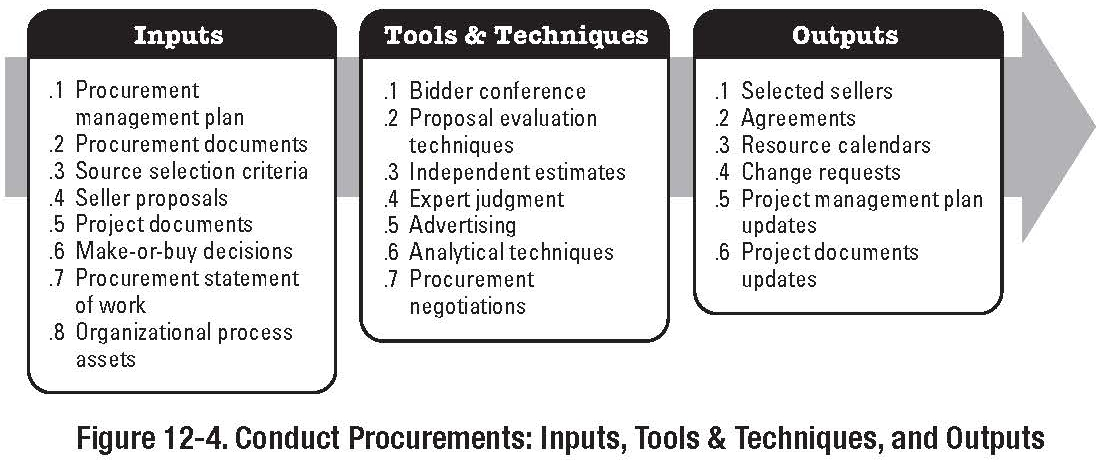
\includegraphics[width = 10cm]{images/Fig12-4.jpg}
	\label{fig:12-4}
\end{figure}
\end{frame}\begin{center}\line(1,0){250}\end{center}




\begin{frame}
\frametitle{Conduct Procurements}
\begin{itemize}
	\item Process of obtaining responses from sellers, such as Quotations, Bids, and Proposals from Prospective Sellers.
	\item Sellers expend most of the effort in this process
	\begin{itemize}
		\item Bidding can be expensive for sellers
		\item Often `quotations' are requested in the very early stages of a project to assist in budget formation. 
	\end{itemize}
\end{itemize}
\end{frame}\begin{center}\line(1,0){250}\end{center}




\begin{frame}
\frametitle{Conduct Procurements \hfill\hfill Inputs}
\textbf{Organisational Process Assets}
		\begin{itemize}
			\item Lists and information on prospective or previously qualified sellers
			\item List should contain information on past performance and other characteristics of the seller
			\item Some organisations only use sellers they have vetted.
			\begin{itemize}
				\item Achilles Supplier Qualification Databases \href{http://www.achilles.ie}{http://www.achilles.ie}
			\end{itemize}
		\end{itemize}
\textbf{Procurement Management Plan}
\begin{itemize}
	\item Refer to book and previous notes
\end{itemize}
\textbf{Procurement Document}s
	\begin{itemize}
		\item Refer to book and previous notes
	\end{itemize}
\end{frame}\begin{center}\line(1,0){250}\end{center}



\begin{frame}
\frametitle{Conduct Procurements \hfill\hfill Tools and Techniques}
\textbf{Bidder Conferences}
	\begin{itemize}
		\item Meetings with prospective sellers prior to preparation of a bid or proposal
		\item Used to ensure all sellers have a clear and common understanding of requirements
		\item In construction a tender procedure is normally followed.
	\end{itemize}
\textbf{Advertising}
\begin{itemize}
	\item Advertising in publications
		\begin{itemize}
			\item \href{http://www.etenders.gov.ie}{http://www.etenders.gov.ie}
		\end{itemize}
\end{itemize}
\textbf{Develop Qualified Sellers List}
\begin{itemize}
	\item Can be done with or without seller involvement
\end{itemize}
\end{frame}\begin{center}\line(1,0){250}\end{center}



\begin{frame}
\frametitle{Conduct Procurements \hfill\hfill Outputs}
\textbf{Qualified Sellers List}\\
\textbf{Procurement Document Package}
		\begin{itemize}
			\item Buyer Prepared Document Package: ITT's Contract, Employers Requirements, General Specification, Particular Specifications, Drawings, Bills, EIS, Ground Investigations, etc.
		\end{itemize}
\textbf{Proposals}
		\begin{itemize}
			\item Seller Prepared Document Package: Form of Tender, Insurance Declarations, Bond Undertakings, Design Documents, Completed Bills, Safety Procedures, Environmental Procedures, Risk Procedures, Methods Statements, Drawings, etc.
			\item Usually Requires Clarification
			\item May also involve interview and/or presentation
		\end{itemize}
\end{frame}\begin{center}\line(1,0){250}\end{center}



\begin{frame}
\frametitle{Selecting Sellers}
Process of Receiving Bids, Proposals, Tenders, etc., and applying evaluation criteria as applicable, to select one or more sellers.\\
\begin{itemize}
	\item Price can be a primary determinant for off the shelf items; 
		\begin{itemize}
			\item but beware, can the seller deliver?
		\end{itemize}
	\item Proposals are normally evaluated under technical and financial criteria
	\item Multiple sources should be considered for critical elements; 
		\begin{itemize}
			\item reduces risk associated with supply
			\item usually costs more in overhead and loss of quantity discounts
		\end{itemize}
\end{itemize}
\end{frame}\begin{center}\line(1,0){250}\end{center}



\begin{frame}
\frametitle{Selecting Sellers \hfill\hfill Tools and Techniques}
\textbf{Weighting System}
\begin{itemize}
	\item Minimise the effect of personal preference or prejudice
	\item Involved assigning a numerical weight to each evaluation criteria, and rating each seller or proposal against these criteria
\end{itemize}
\textbf{Independent Estimates}
\begin{itemize}
	\item AKA `should-cost' estimate
	\item Significant deviation from this estimate gives an indication that something is wrong.. Either with the proposal or the request
\end{itemize}
\textbf{Screening System}
\begin{itemize}
	\item Minimum criteria that must be met prior to consideration of the proposal;  Annual Turnover, Number of Employees, H\&S History, etc.
\end{itemize}
\end{frame}\begin{center}\line(1,0){250}\end{center}


\begin{frame}
\frametitle{Selecting Sellers \hfill\hfill Tools and Techniques}
\textbf{Contract Negotiation}
\begin{itemize}
	\item Clarifies structure and requirements for the contract
	\item Responsibilities, applicable laws and language, financing, etc. 
\end{itemize}
\textbf{Seller Rating System}
\begin{itemize}
	\item Records of Sellers past performance
	\item Quality, Delivery Performance, Contractual Compliance, etc.
\end{itemize}
\end{frame}\begin{center}\line(1,0){250}\end{center}



\begin{frame}
\frametitle{Selecting Sellers \hfill\hfill Tools and Techniques}
\textbf{Expert Judgment}
\begin{itemize}
	\item Multi-Discipline Review Team
	\item Legal, Financial, Technical, etc.
	\item Team prepares report on proposal and makes recommendations
\end{itemize}
\textbf{Proposal Evaluation Techniques}
\begin{itemize}
	\item Weighting Systems et. al. 
\end{itemize}
\end{frame}\begin{center}\line(1,0){250}\end{center}


\begin{frame}
\frametitle{NRA Pavements and Minor Works Contracts}
\begin{figure}
	\centering
		\includegraphics[width = 10cm]{images/prequal.jpg}
	\label{fig:prequal1}
\end{figure}
\end{frame}\begin{center}\line(1,0){250}\end{center}
This text was taken from a pre-qualification document produced by the NRA. 


\begin{frame}
\frametitle{NRA Pavements and Minor Works Contracts}
\begin{figure}
	\centering
		\includegraphics[width = 10cm]{images/prequal2.jpg}
	\label{fig:prequal2}
\end{figure}
\end{frame}\begin{center}\line(1,0){250}\end{center}
Section (a) contains an error.  \euro1.0M annual turnover is required in figures whereas \euro800k is required in words.  Which one will apply?  The criteria under (c) is also of interest.  The candidate must have at least three employees for every \euro1.3M of turnover.   


\begin{frame}
\frametitle{NRA Pavements and Minor Works Contracts}
\begin{figure}
	\centering
		\includegraphics[width = 8cm]{images/prequal3.jpg}
	\label{fig:prequal3}
\end{figure}
\end{frame}\begin{center}\line(1,0){250}\end{center}


\begin{frame}
\frametitle{Selecting Sellers \hfill\hfill Outputs}
\textbf{Selected Sellers}
		\begin{itemize}
			\item Those sellers judged/determined to be within competitive range
		\end{itemize}
\textbf{Contract}
		\begin{itemize}
			\item May be a complex contract or a PO
		\end{itemize}
\textbf{Contract Management Plan}
		\begin{itemize}
			\item Plan to administer the contract
			\begin{itemize}
				\item Who, What, When, etc; Resource Availability
				\item Procurement Management Plan (Updates)
				\item Requested Changes
			\end{itemize}
		\end{itemize}			
\end{frame}\begin{center}\line(1,0){250}\end{center}



\begin{frame}
\frametitle{Select Sellers \hfill\hfill Outputs}
\textbf{Contract (cont.):} \\
May contain the following elements (no specific order):
\begin{footnotesize}
\begin{table}[htb]
	\centering
		\begin{tabular}{|l|l|l|}
			\hline
			Section Headings	&	Statement of Work	&	Schedule\\
			\hline			
			Period of Performance	&	Roles \& Responsibilities	&	Pricing \& Payment\\
			\hline			
			Inflation Adjustments	&	Acceptance Criteria	&	Warranty\\
			\hline			
			Product Support	&	Limitation of Liability	&	Fees\\
			\hline
			Retention	&	Penalties \& Incentives	&	Insurances\\
			\hline
			Performance Bonds	&	Subcontractor Approval	&	Change Request\\
				&		&	Handling\\
			\hline
			Termination and 	&		&	\\
			Dispute Handling Procedures	&		&	\\
			\hline
		\end{tabular}
\end{table}
\end{footnotesize}
\end{frame}\begin{center}\line(1,0){250}\end{center}




\subsection{Administer Procurements}

\begin{frame}
\frametitle{Administer Procurements}
\textbf{Part of the Monitoring and Controlling Process Group}
\begin{figure}
	\centering
		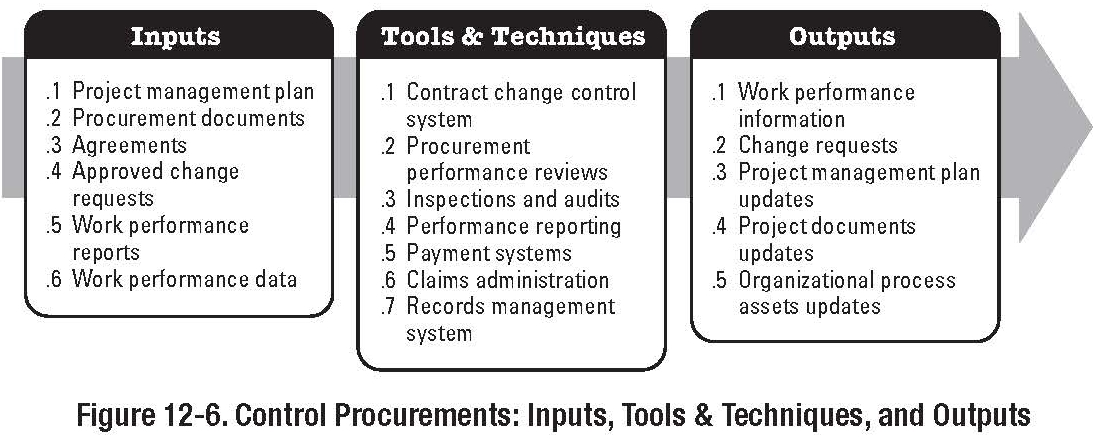
\includegraphics[width = 10cm]{images/Fig12-6.jpg}
	\label{fig:12-6}
\end{figure}

\end{frame}\begin{center}\line(1,0){250}\end{center}


\begin{frame}
\frametitle{Contract Administration}
\begin{itemize}
	\item Each party to a contract needs to ensure that they are meeting their own contractual obligations, and that the other party is meeting theirs.
	\item Both parties need to ensure that their own legal rights are being protected
	\item The legal nature of contractual relationships makes it vital that the project management team is acutely aware of the legal implications of actions taken when administering contracts
\end{itemize}
\end{frame}\begin{center}\line(1,0){250}\end{center}




\begin{frame}
\frametitle{Contract Administration}
Due to legal considerations, many organisations will treat contract administration as an administrative function.\\
\begin{itemize}
	\item The `contract administrator' may or may not be part of the project team
	\item This can lead to difficulty for the project management team
\end{itemize}
Contract Administration also has a financial component; monitoring payments made to the seller (such as a sub-contractor)
\begin{itemize}
	\item Must ensure payments are within the terms defined by the contract, and that `payment certification' is appropriate
\end{itemize}
\end{frame}\begin{center}\line(1,0){250}\end{center}



\begin{frame}
\frametitle{Contract Administration}
Contract Administration also reviews and documents how a seller is performing, or has performed, based on the contract and established corrective actions
\begin{itemize}
	\item Determine sellers competency or lack of competency
Contract Administration includes managing early termination of contract
	\item Usually difficult to terminate a contract
	\item Limerick City Council v. Uniform Construction Limited: Clear grounds for termination must be established 
\end{itemize}
\end{frame}\begin{center}\line(1,0){250}\end{center}



\begin{frame}
\frametitle{Contract Administration}
\textbf{BEWARE:}
\textit{Modification of Contract by Mutual Consent}
\begin{itemize}
	\item Minutes of Meetings, Memo's, supposedly benign offers can, in effect, modify the contract.
	\item Usually caused by variations, or changes in scope, etc.
\end{itemize}
Project Management Team must fully investigate the impact of variations, or changes in scope. 
\end{frame}\begin{center}\line(1,0){250}\end{center}



\begin{frame}
\frametitle{Administer Procurements \hfill\hfill Inputs}

\begin{itemize}
	\item Procurement Documents
	\item Project Management Plan
	\item Contract
	\item Performance Reports
	\item Seller Related Performance Documentation includes:
		\begin{itemize}
			\item Seller-developed technical documentation and other deliverables information developed in accordance with the contract
				\item Seller Performance Reports
				\item Approved Change Requests
				\item Work Performance Information
		\end{itemize}
\end{itemize}
\end{frame}\begin{center}\line(1,0){250}\end{center}




\begin{frame}
\frametitle{Administer Procurements \hfill\hfill Inputs}
\textbf{Approved Change Requests}
	\begin{itemize}
		\item Approved Change Requests can include modifications to the contract: Scope, Spec, Price, Time, etc.
		\item Beware of Verbal Changes or Aggreements - Can modify the contract by mutual consent if it is recorded; including notes in a diary.
	\end{itemize}
\textbf{Work Performance Information}
		\begin{itemize}
			\item Extent to which quality standards are being met
			\item	Costs / Certificates to date
			\item	Deliverables Status
			\item Build in status reporting into contact, AND payment mechanism.
		\end{itemize}
\end{frame}\begin{center}\line(1,0){250}\end{center}




\begin{frame}
\frametitle{Administer Procurements \hfill\hfill Tools and Techniques}
\textbf{Contract Change Control System}
		\begin{itemize}
			\item Defines the process by which the contract can be modified: May include review by lawyer, etc.
		\end{itemize}
\textbf{Buyer Conducted Performance Review}
		\begin{itemize}
			\item Performance Review is a structured review to determine the sellers progress to deliver project scope and quality, within cost and schedule, as compared to the contract
		\end{itemize}
\textbf{Inspections and Audits}
\begin{itemize}
			\item Conducted by the buyer during the course of the contract to identify any weaknesses in the sellers work processes or deliverables
		\item Inspections and Audits should be built into the contact 
		\end{itemize}
\end{frame}\begin{center}\line(1,0){250}\end{center}





\begin{frame}
\frametitle{Administer Procurements \hfill\hfill Tools and Techniques}
\textbf{Performance Reporting}
		\begin{itemize}
			\item Provides management with information about how effectively the seller is achieving the contractual objectives
		\end{itemize}
\textbf{Payment System}
		\begin{itemize}
			\item Payment system includes appropriate reviews and approvals
			\item Must be made in accordance with the contract
		\end{itemize}
\textbf{Claims Administration}
		\begin{itemize}
			\item Contested and Constructive Changes
			\item PMBOK\textregistered refers to `Claims' as being contested, or not agreed by the parties
		\end{itemize}
\textbf{Litigation, Arbitration, etc.}
		\begin{itemize}
			\item Normal `Variations' are not considered part of this
			\item `Claims' must follow the dispute procedure as set down in the contract.
		\end{itemize}
\end{frame}\begin{center}\line(1,0){250}\end{center}




\begin{frame}
\frametitle{Administer Procurements \hfill\hfill Tools and Techniques}
\textbf{Records Management System}
\begin{itemize}
	\item Part of the Project Management Information system
	\item Indexing of Project Documentation and Records
\end{itemize}
\textbf{Information Technology}
\begin{itemize}
	\item Use of Information Technology and Communications Technologies to enhance the efficiency and effectiveness of contract administration
\item Payment Systems, Databases, etc.
\end{itemize}
\end{frame}\begin{center}\line(1,0){250}\end{center}



\begin{frame}
\frametitle{Administer Procurements \hfill\hfill Tools and Techniques}

Information Technology (cont.)
\begin{itemize}
	\item Biometric Information Systems
\end{itemize}
Site Access Control and Monitoring
Donseed: Biometric Access systems etc.


\href{http://www.donseed.com}{http://www.donseed.com}
\begin{figure}
	\centering
		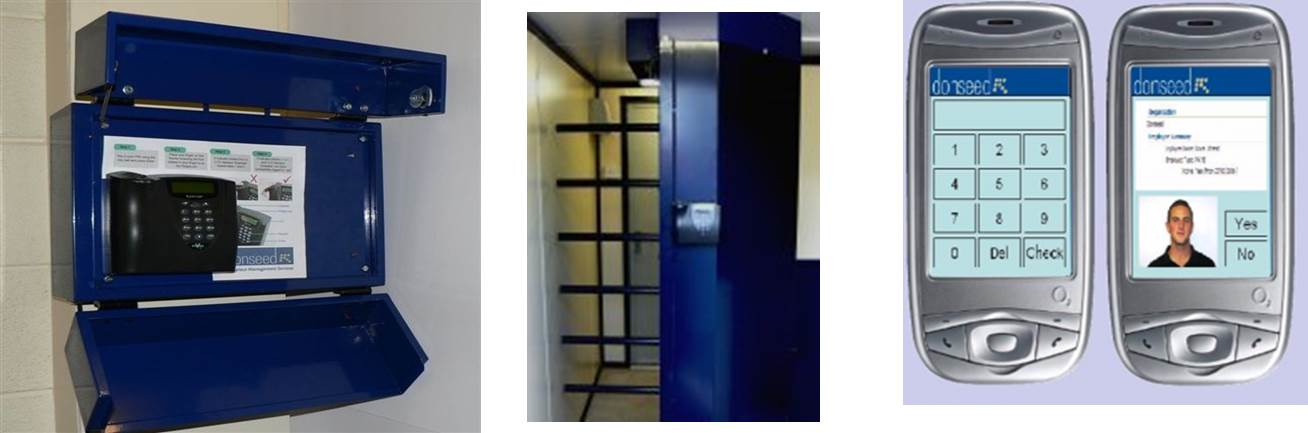
\includegraphics[width = 7cm]{images/donseed.jpg}
	\label{fig:donseed}
\end{figure}
\end{frame}\begin{center}\line(1,0){250}\end{center}




\begin{frame}
\frametitle{Administer Procurements \hfill\hfill Outputs}

\textbf{Procurement Documentation}
\begin{itemize}
	\item Contract, and Supporting Documentation, etc.
\end{itemize}
\textbf{Organisational Process Assets Updates}
		\begin{itemize}
			\item Correspondence
			\item Payment Schedules and Requests
			\item Seller Performance Evaluation Documentation
		\end{itemize}
\textbf{Change Requests}\\
\textbf{Project Management Plan Updates}
		\begin{itemize}
			\item Procurement Management Plan
			\item Baseline Schedule
		\end{itemize}
\end{frame}\begin{center}\line(1,0){250}\end{center}



\subsection{Close Procurements}

\begin{frame}
\frametitle{Close Procurements}
\textbf{Part of the Closing Process Group}
\begin{figure}
	\centering
		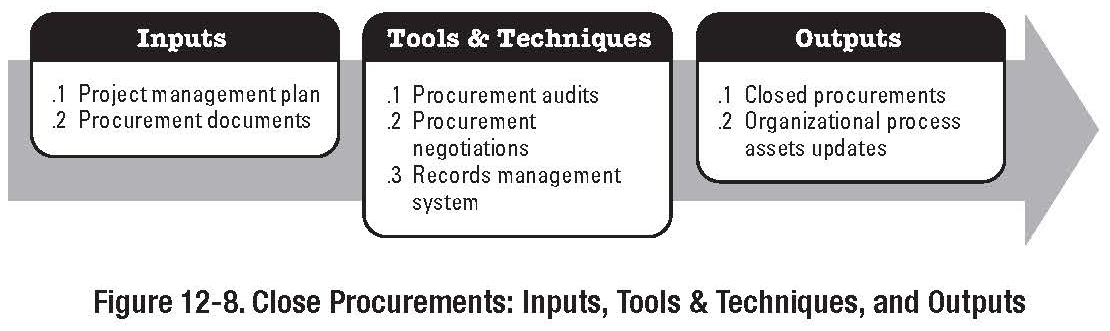
\includegraphics[width = 10cm]{images/Fig12-8.jpg}
	\label{fig:12-8}
\end{figure}

\end{frame}\begin{center}\line(1,0){250}\end{center}





\begin{frame}
\frametitle{Close Procurements}
\begin{itemize}
	\item Contract Closure Supports the `Close Project or Phase' process
	\item Involves verification that all work and deliverables were acceptable
	\item Also involves administrative work such as:
		\begin{itemize}
			\item Updating records to reflect final results
			\item Archiving information for future use
		\end{itemize}
\item May also involve unresolved claims and disputes
\item Contracts can also be closed by mutual agreement
		\begin{itemize}
			\item Not the same as termination or discharge
		\end{itemize}
\end{itemize}
\end{frame}\begin{center}\line(1,0){250}\end{center}




\begin{frame}
\frametitle{Close Procurements  \hfill\hfill Inputs}
\begin{itemize}
	\item Project Management Plan
	\item Procurement Documentation
\end{itemize}
\textbf{Tools and Techniques}
\begin{itemize}
	\item Procurement Audits
	\item Negotiated Settlements
	\item Records Management System
\end{itemize}
\end{frame}\begin{center}\line(1,0){250}\end{center}






\begin{frame}
\frametitle{Close Procurements  \hfill\hfill Outputs}
\textbf{Closed Procurements}
		\begin{itemize}
			\item Buyer provides seller with formal notification of completion of contract; TOC, etc.
		\end{itemize}
\textbf{Organisational Process Assets}
	\begin{itemize}
		\item Contract File
		\item Deliverable Acceptance
		\item Lessons Learned Documentation
	\end{itemize}
\end{frame}\begin{center}\line(1,0){250}\end{center}




%% END OF LECTURE SLIDE
\begin{frame}
\frametitle{Next Lecture}{Reading:}
`A Guide to the Project Management Body of Knowledge'\\ 
Chapter 10 - Project Communications Management
\begin{figure}[h]
	\centering
		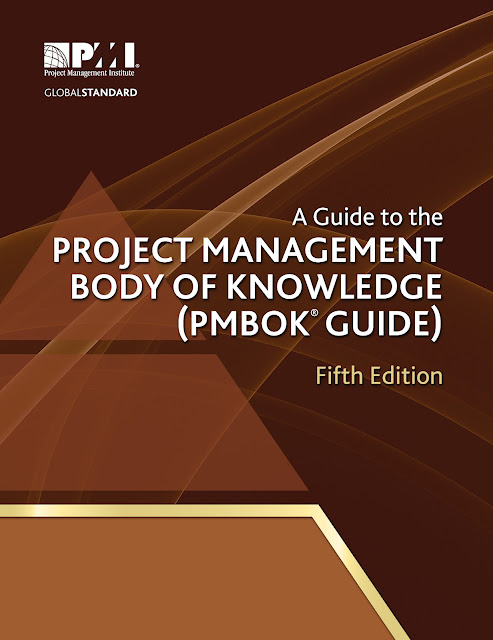
\includegraphics[width = 4cm]{images/book.jpg}
\end{figure}
\end{frame}\begin{center}\line(1,0){250}\end{center}
%% END OF LECTURE SLIDE



\end{document}


\end{center}